% Bsp. eines Hauptteils

\chapter{Ziel des Projekts}
\label{sec:grundl}
Ziel des Projektes ist es, eine Software zu entwickeln, die den File-IO von Anwendungen analysiert. Die Software soll sich dabei zwischen das zu analysierende Programm und das Betriebssystem schalten und s\"amtlichen File-IO abfangen. Der File-IO des Programms soll anschliessend gespeichert und graphisch aufbereitet werden. Die Software soll dabei interaktiv sein. Das bedeutet, es soll mit der Software m\"oglich sein, gezielt nach IO-Engp\"assen in einer Anwendung zu suchen.\newline\newline
Ziel ist es dar\"uber hinaus, mit der Software ein Framework zur Analyse von File-IO zu schaffen. Dies bedeutet, dass es m\"oglich sein soll, die Software so zu erweitern, dass mit ihr nicht nur POSIX-IO und MPI-IO, sondern z.B. auch das parallele Dateisystem Lustre analysiert werden kann.\newline\newline
Im ersten Schritt sollen dabei bestehende Softwarel\"osungen evaluiert werden. Im zweiten Schritt geht es dann darum, eine eigene Software zu entwickeln, welche die oben genannten Forderungen erf\"ullt. Die Entwicklung der Software soll dabei portabel mit CMake erfolgen. Die Software soll dar\"uber hinaus Thread-Sicherheit haben. Dies bedeutet, dass sie von mehreren Threads zugleich bedient werden kann. Die Visualisierung soll zudem portabel sein. Die generierten Daten \"uber den File-IO sollen also plattformunabh\"angig bspw. \"uber einen Webserver visualisiert werden k\"onnen.

\chapter{Stand der Technik}
\label{sec:tech}
Im Rahmen der Forschungsarbeit erfolgte zun\"achst eine Marktrecherche, welche Softwarel\"osungen zum Tracing von File-IO bereits auf dem Markt sind. Die L\"osungen, welche den Anforderungen dieses Projektes am ehesten entsprechen wurden dar\"uber hinaus bez\"uglicher ihrer Funktionalit\"at evaluiert. Als wichtigstes Kriterium gilt hierbei, dass es mit der Software sowohl m\"oglich ist POSIX-IO zu untersuchen, als auch MPI-IO. Dar\"uber hinaus soll die Analyse zur Laufzeit ohne Rekompilieren des Codes m\"oglich sein. Dies soll sowohl f\"ur statisch als auch f\"ur dynamisch gelinkte Programme der Fall sein.
\section{Darshan}
Darshan ist ein Programm zur Analyse von POSIX-IO und MPI-IO. Mit Darshan kann ein PDF-Report des File-IOs von Anwendungen erstellt werden. Bei dynamisch gelinkten Programmen ist dies zur Laufzeit m\"oglich, bei statisch gelinkten Programmen ausschliesslich beim Bau des Programms.\newline
Darshan besteht dabei aus zwei Programmen. Mit Darshan-Runtime werden die Informationen \"uber den File-IO eines Programms ermittelt und in einer Log-Datei gespeichert. Die Daten in der Log-Datei k\"onnen anschliessend mit Darshan-Util dargestellt und analysiert werden.
\subsection{Funktionsweise}
Das Sammeln von Informationen zur Laufzeit von Programmen geschieht \"uber die Systemvariable LD\_PRELOAD. Mit dieser ist es m\"oglich Features in ein Prorgamm einzuschleusen. Beim Laden von Shared Libraries wird dabei zun\"achst nicht die eigentliche Bibliothek geladen, sondern diese, welche unter LD\_PRELOAD angegeben wurde. Damit wird dann die Darshan-Bibliothek geladen, welche die IO-Befehle speichert und diese anschliessend an die eigentlichen Bibliotheken weitergibt. Die Funktionsweise von Darshan f\"ur dynamisch gelinkte Programme ist in Abbildung \ref{fig:darshan} dargestellt. Die Bibliothek libdarshan.so wird dabei vom zu untersuchenden Programm \"uber LD\_PRELOAD geladen. Diese speichert alle MPI-IO- und POSIX-IO-Befehle in Log-Dateien. Diese Log-Dateien k\"onnen anschliessend mit Darshan-Util ausgewertet werden. Dabei wird entweder ein PDF-Report kreiert in welchem in Diagrammen u.a. dargestellt wird, wieviele File-IO-Operationen jeweils durchgef\"uhrt wurden und welche Datenmengen dabei verarbeitet wurden. Alternativ k\"onnen die Informationen in eine Textdatei geschrieben und \"uber die Kommandozeile ausgegeben werden.

\begin{figure}[h]
	\centering
	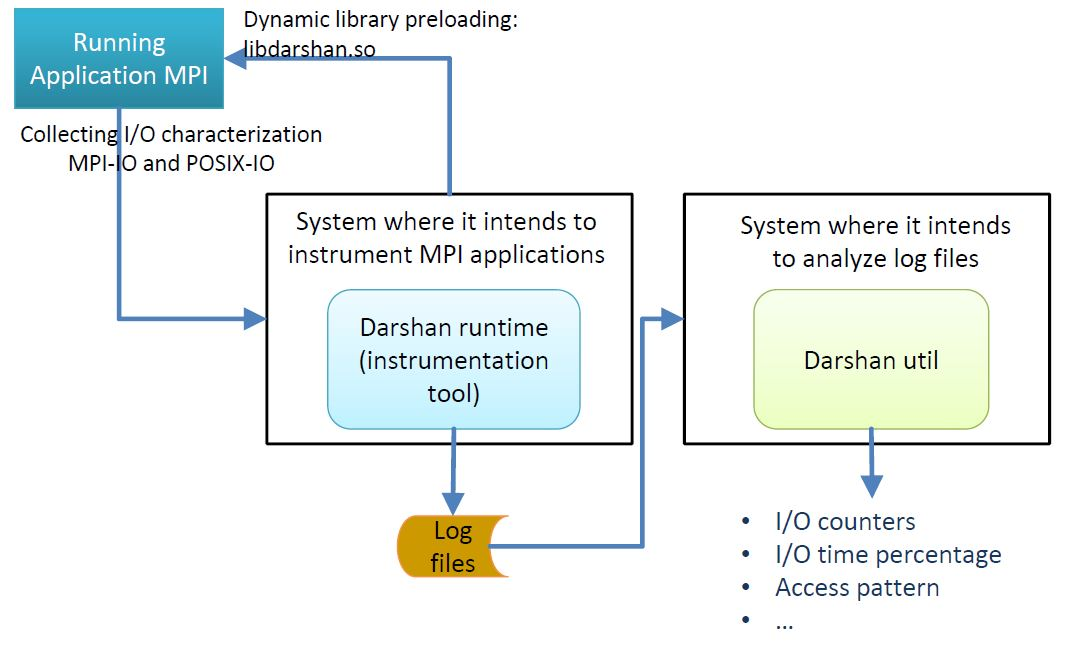
\includegraphics[width=12cm]{fig/Darshan.jpg}
	\caption{Darshan Aufbau \cite{Mendez.23.06.2016}}
	\label{fig:darshan}
\end{figure}

Das Analysieren von statisch gelinkten Programmen funktioniert \"ahnlich zu VampirTrace mit Compiler-Wrappern. Diese werden beim Bau anstatt der eigentlichen Compiler aufgerufen. Die Wrapper rufen dabei die eigentlichen Compiler auf, erweitern jedoch das zu kompilierende Programm so, dass es mit Darshan analysiert werden kann. \cite{ArgonneNationalLaboratory.22.01.2019}\cite{ArgonneNationalLaboratory.19.01.2019}
\subsection{Fazit}
Darshan ist ein hervorragendes Programm zur Analyse des IO von dynamisch gelinkten Programmen. Der Nachteil liegt dabei jedoch darin, dass der graphische Output nicht interaktiv ist. Es wird zwar ein PDF-Report kreiert, es ist jedoch nicht m\"oglich interaktiv gezielt nach Schwachstellen im Programm zu suchen. Dar\"uber hinaus k\"onnen statisch gelinkte Programme mit Darshan nicht zur Laufzeit ohne erneuten Bau untersucht werden, was ebenfalls einen gravierenden Nachteil darstellt. 
\section{VampirTrace}
VampirTrace ist ein Programm, welches von der Universit\"at Dresden urspr\"unglich zur Analyse von MPI-Programmen entwickelt wurde. Mittlerweile ist es ein Tool-Set zur Analyse von parallelen Programmen im HPC-Bereich. Mit VampirTrace k\"onnen sowohl MPI-IO als auch POSIX-IO untersucht werden. F\"ur die Analyse von Programmen ist es notwendig, diese mithilfe von VampirTrace-Compiler-Wrappern neu zu bauen. Im Makefile m\"ussen dabei die Compiler durch die Compiler-Wrapper von VampirTrace ersetzt werden. Diese rufen dann wiederum die eigentlichen Compiler auf. Die gebauten Programme k\"onnen anschliessend zur Laufzeit mit VampirTrace analysiert werden. Eine Untersuchung zur Laufzeit ohne erneuten Bau ist nicht ohne weiteres m\"oglich.\newline\newline
Die gewonnenen Daten werden von VampirTrace in einer Log-Datei im Open-Trace-Format (OTF) gespeichert. Diese Log-Dateien k\"onnen anschliessend mit Tools, die den Umgang mit OTF beherrschen, visualisiert werden. Am besten eignet sich hierzu das Tool Vampir, welches ebenfalls von der Universit\"at Dresden zu diesem Zweck entwickelt wurde. Mit diesem Tool ist es m\"oglich Daten im OTF-Format interaktiv zu visualisieren und damit gezielt nach Schwachstellen zu suchen.
\cite{TUDresden.2016}\cite{Mendez.23.06.2016}
\section{Score-P}
Score-P ist eine Software, die als Nachfolger von VampirTrace entwickelt wurde. In der Funktionsweise ist Score-P VampirTrace dabei recht \"ahnlich. Die Daten werden ebenfalls im OTF-Format gespeichert und k\"onnen mit VampirTrace visualisiert werden. Alternativ k\"onnen die Daten jedoch auch im TAU-Format gespeichert und mit der Software TAU analysiert werden, welche im n\"achsten Abschnitt erl\"autert wird. F\"ur die Analyse von File-IO ist VampirTrace aber nach wie vor die bessere Alternative.\cite{Kunke.2014}\cite{VirtualInstituteHighProductivitySupercomputing.2018}
\begin{figure}[h]
	\centering
	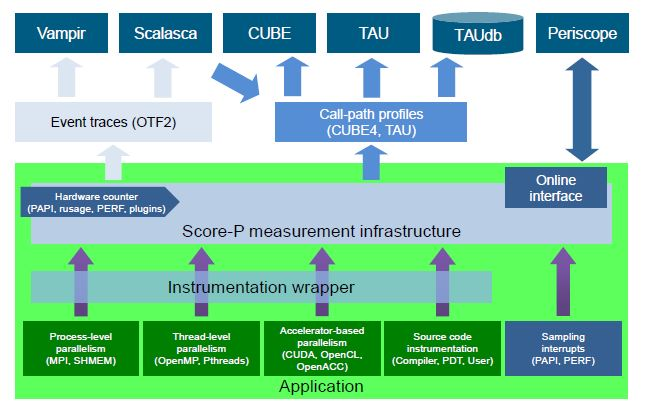
\includegraphics[width=12cm]{fig/Score-P.jpg}
	\caption{Score-P \cite{VirtualInstituteHighProductivitySupercomputing.2018}}
	\label{fig:score-p}
\end{figure}
\section{Ludalo}
Mit Ludalo ist es m\"oglich, Lustre-Metadaten-Operationen zu analysieren. Dies kann in diesem Projekt im weiteren Verlauf erforderlich sein, wenn die Funktionalit\"at der entwickelten Software f\"ur Lustre erweitert werden soll. Lustre ist dabei ein paralleles Dateisystem, welches haupts\"achlich im HPC-Bereich eingesetzt wird.
\cite{Berger.30.07.2014}
\section{TAU}
Tau ist eine Software, entwickelt von der University of Oregon, zur Analyse von parallelen Applikationen. Eine File-IO-Analyse ist dabei sowohl f\"ur POSIX-IO, als auch f\"ur MPI-IO m\"oglich. Die von TAU generierten Daten k\"onnen im OTF-Format gespeichert und anschliessend mit Vampir visualisiert werden. Damit \"ähnelt TAU stark VampirTrace, wo die Daten ebenfalls mit Vampir visualisiert werden k\"onnen. Die Analyse der Programme erfolgt entweder durch das Recompilieren des Quelltextes oder durch das Laden einer Bibliothek mit LD\_PRELOAD, was jedoch nur bei dynamisch gelinkten Programmen m\"oglich ist. Dies stellt auch den entscheidenden Vorteil von TAU gegen\"uber VampirTrace dar. Die Visualisierung ist bei beiden Tools identisch, allerdings k\"onnen mit TAU dynamisch gelinkte Programme ohne Rekompilieren analysiert werden.
\cite{Shende.03.05.2017}\cite{Shende.2011}\cite{UniversityofOregon.2018}

\section{Fazit}
Keines der untersuchten Programme enth\"alt alle Features, welche in diesem Projekt gew\"unscht sind. Diese sind in Tabelle \ref{tab:Recherche} vergleichend dargestellt.
\begin{table}[h]
	\centering
	\begin{tabular}{l|l|l|l}
		\textbf{} & \textbf{Darshan} & \textbf{VampirTrace}& \textbf{TAU}\\
		\hline
		\textbf{Analyse von POSIX-IO} & + & + & + \\
		\hline
		\textbf{Analyse von MPI-IO} & + & + & + \\
		\hline
		\textbf{Interaktive Bedienung}& - & + & + \\
		\hline
		\textbf{dynamisch gelinkte Programme} & + & - & + \\
		\hline
		\textbf{statisch gelinkte Programme} & - & - & - \\
		\hline
		\textbf{Schwerpunkt auf File-IO-Analyse} & + & - & - \\
	\end{tabular}
	\caption{Marktrecherche}
	\label{tab:Recherche}
\end{table}
Die Analyse von POSIX-IO und MPI-IO ist mit allen untersuchten Produkten m\"oglich. Hinsichtlich der Visualisierung sind sich VampirTrace und TAU \"ahnlich. Bei beiden werden die Daten im OTF-Format gespeichert und k\"onnen mit Vampir untersucht werden, womit auch eine interaktive Bedienung m\"oglich ist. Mit Darshan k\"onnen zwar ebenfalls POSIX-IO und MPI-IO analysiert werden, allerdings kann die Visualisierung durch den PDF-Report oder eine Textdatei nicht interaktiv bedient werden. Der entscheidende Vorteil von Darshan gegen\"uber den anderen Tools ist jedoch, dass es ausschliesslich f\"ur die Analyse von File-IO entwickelt wurde und dadurch deutlich leichtgewichtiger ist.\newline
Die Schwachstelle der Produkte liegt in der Analyse von statisch gelinkten Programmen. Dies ist zwar prinzipiell bei allen m\"oglich, jedoch nur durch das erneute Kompilieren des Quelltextes. Aus diesem Grund soll in diesem Projekt eine eigene Software entwickelt werden, bei welcher dies m\"oglich ist und welche eine interaktive Visualisierung beinhaltet.

\chapter{Entwicklung einer eigenen Software}
\section{Architektur}
\label{sec:real}

\section{Umsetzung}
\label{sec:umsetz}

\chapter{Aktueller Stand}
\label{sec:ergeb}

